\chapter{Test Journal: DC motor torque constant $\boldsymbol{K_t}$ and friction coefficient $\boldsymbol{B_m}$}\label{appendix:TJDCMotorTorqueConstant}
\begin{table}[!h]
\begin{tabular}{l l}
\textbf{Test participants:} & Maxime \& Robin\\
\textbf{Date:}  & 24/10-2016
\end{tabular}
\end{table}

\section*{Purpose}
The purpose of the test is to determine the motor torque constant $K_t$ and the friction coefficient $B_m$ of the DC motor on the motorised antenna stand. A measurements has to be done to determine $K_t$, afterwards $B_m$ can be calculated using the value of $K_t$ and the results from \autoref{test:Ke}.

\section*{Test equipment and components}
The test equipment and components are listed in \autoref{tab_appendix:testKt}.
\begin{table}[!h]
	\centering
	\caption{List of measurement equipment and components}\label{tab_appendix:testKt}

	\begin{tabularx}{\textwidth}{lXXXX}
		Name 				& Brand	& Model & AAU-number\\ \toprule \rowcolor{lightGrey}
		Oscilloscope	& Agilient technologies & DSO6034A & 60763	\\
		Powersupply	& Hameg & HM7042-5 & 61597\\ \rowcolor{lightGrey}
		Powersupply	& Hameg & HM7042-3 & 61597\\ 
		DC motor & Maxon & 41.023.038-00.00-052& N/A \\ \rowcolor{lightGrey}
		Multimeter & Fluke & 37 & 33019 \\
		Torque sensor & ICom & MWA-W8-1-P & 08931 \\ \rowcolor{lightGrey}
		Torque meterbox & N/A & N/A & N/A 
	\end{tabularx}
\end{table}

\section*{Setup}
Diagram of the setup to measure $K_t$ is illustrated on \autoref{fig:DCR_Ktcircuit}. 
\begin{figure} [!h]
    \centering
        \includegraphics[width=\textwidth]{figures/test/DCR_Ktcircuit}
        \caption{Diagram of the setup. Oscilloscope icon is from \cite{web:OscilloscopeIcon}}
        \label{fig:DCR_Ktcircuit}
\end{figure}

The motors rotor shaft is fastened to the torque sensor, and the torque sensors rotary body is fastened in place. The torque sensor is connected to a voltage source of \SI{12}{\volt} to \SI{16}{\volt} as stated on the torque sensor. The DC motor is connected to a voltage source through an amp-meter. 
\begin{enumerate}
\item Set the voltage supply at a certain voltage
\item Wait for system to reach steady state
\item Read current and output of the torque sensor
\item Repeat steps 1 to 3 at different supply voltages
\end{enumerate}

\section*{Results}
The results from the test are listed in \autoref{tab_appendix:testKe}
\begin{table} [!h]
	\centering
	\caption{Data of the measurement}\label{tab_appendix:testKe}
	\begin{tabularx}{\textwidth}{XX}
		Current, $i_a$ [\si{\ampere}]& Torque sensor voltage, $v_\tau$ [\si{\volt}]								\\ \toprule \rowcolor{lightGrey}
		0.052 & 0.136 \\
		0.100	& 0.213 \\ \rowcolor{lightGrey}
		0.149 & 0.303 \\
		0.152 & 0.345\\\rowcolor{lightGrey}
		0.188 & 0.405\\
		0.193 & 0.443\\\rowcolor{lightGrey}
		0.197 & 0.416 \\
		0.249 & 0.523 \\ \rowcolor{lightGrey}
		0.297 & 0.619 
	\end{tabularx}
\end{table}

\section*{Data processing}
The data processing is split into two parts. Derivation of $K_t$ and calculation of $B_m$. $K_t$ will be determined first.

\subsection*{Determining $\boldsymbol{K_t}$}
The DC motor can, as mentioned in \autoref{sec:DC-motorTechnicalKnowledge}, be described by \autoref{eq:AppendixDCMotorDiffEquation}:
\begin{equation}\label{eq:AppendixDCMotorDiffEquation}
J_m \cdot \frac{d\omega_{m}(t)}{d t} = \tau_{m}(t) - \tau_{l}(t) - B_m \cdot \omega_{m}(t)	\addunit{\newton\metre}
\end{equation}
\startexplain
\explain{$J_m$ is moment of inertia of the rotor shaft}{\si{\newton\metre\second\squared\per\radian}}
\explain{$B_m$ is the motors dampening constant}{\si{\newton\metre\second\per\radian}}
\explain{$\tau_m(t)$ is the torque applied by the motor}{\si{\newton\metre}}
\explain{$\tau_l(t)$ is the torque applied by the load}{\si{\newton\metre}}
\explain{$\omega_m(t)$ is the rotational speed of the rotor shaft}{\si{\radian\per\second}}
\stopexplain

By applying $\omega_m(t)=0$, \autoref{eq:AppendixDCMotorTorque} can be derived.
\begin{equation}\label{eq:AppendixDCMotorTorque}
J_m \cdot 0 = \tau_{m}(t) - \tau_{l}(t) - B_m \cdot 0 \implies \tau_{m}(t) = \tau_{l}(t) \addunit{\newton\metre}
\end{equation}

The torque $\tau_{m}(t)$ applied by the motor is given by the current through the DC motor multiplied with the proportionality factor $K_t$, as seen in \autoref{eq:AppendixDCMotorKtProportionality}.
\begin{equation}\label{eq:AppendixDCMotorKtProportionality}
\tau_{m}(t)= \tau_l(t) = i_a(t) \cdot K_t \implies K_t = \frac{\tau_{l}(t)}{i_a(t)} \addunit{\newton\metre\per\ampere}
\end{equation}
\startexplain
\explain{$i_a(t)$ is the current through the DC motor}{\si{\ampere}}
\explain{$K_t$ is the DC motor torque constant}{\si{\newton\metre\per\ampere}}
\stopexplain

Hereby it is concluded that the DC motor torque constant can be derived by locking the DC motor rotor shaft in place, and measuring the torque applied to the locking mechanism and the current through the DC motor.

The output of the torque sensor $v_\tau(t)$ in respect to the actual torque is given by \autoref{eq:AppendixDCMotorSensorConstant}.
\begin{equation}
v_\tau(t) = \tau_{l}(t) \cdot 5 \implies \tau_{l}(t) = \frac{v_\tau(t)}{5} \addunit{\newton\metre}\label{eq:AppendixDCMotorSensorConstant}
\end{equation}
\startexplain
\explain{$v_\tau(t)$ is the output of the torque sensor}{\si{\volt}}
\stopexplain

The torque sensor torque $\tau_l(t)$ is plotted with respect to the current $i_a(t)$ in \autoref{fig:DCMotorKtMeasurement}.
\begin{figure}[!h]
\centering
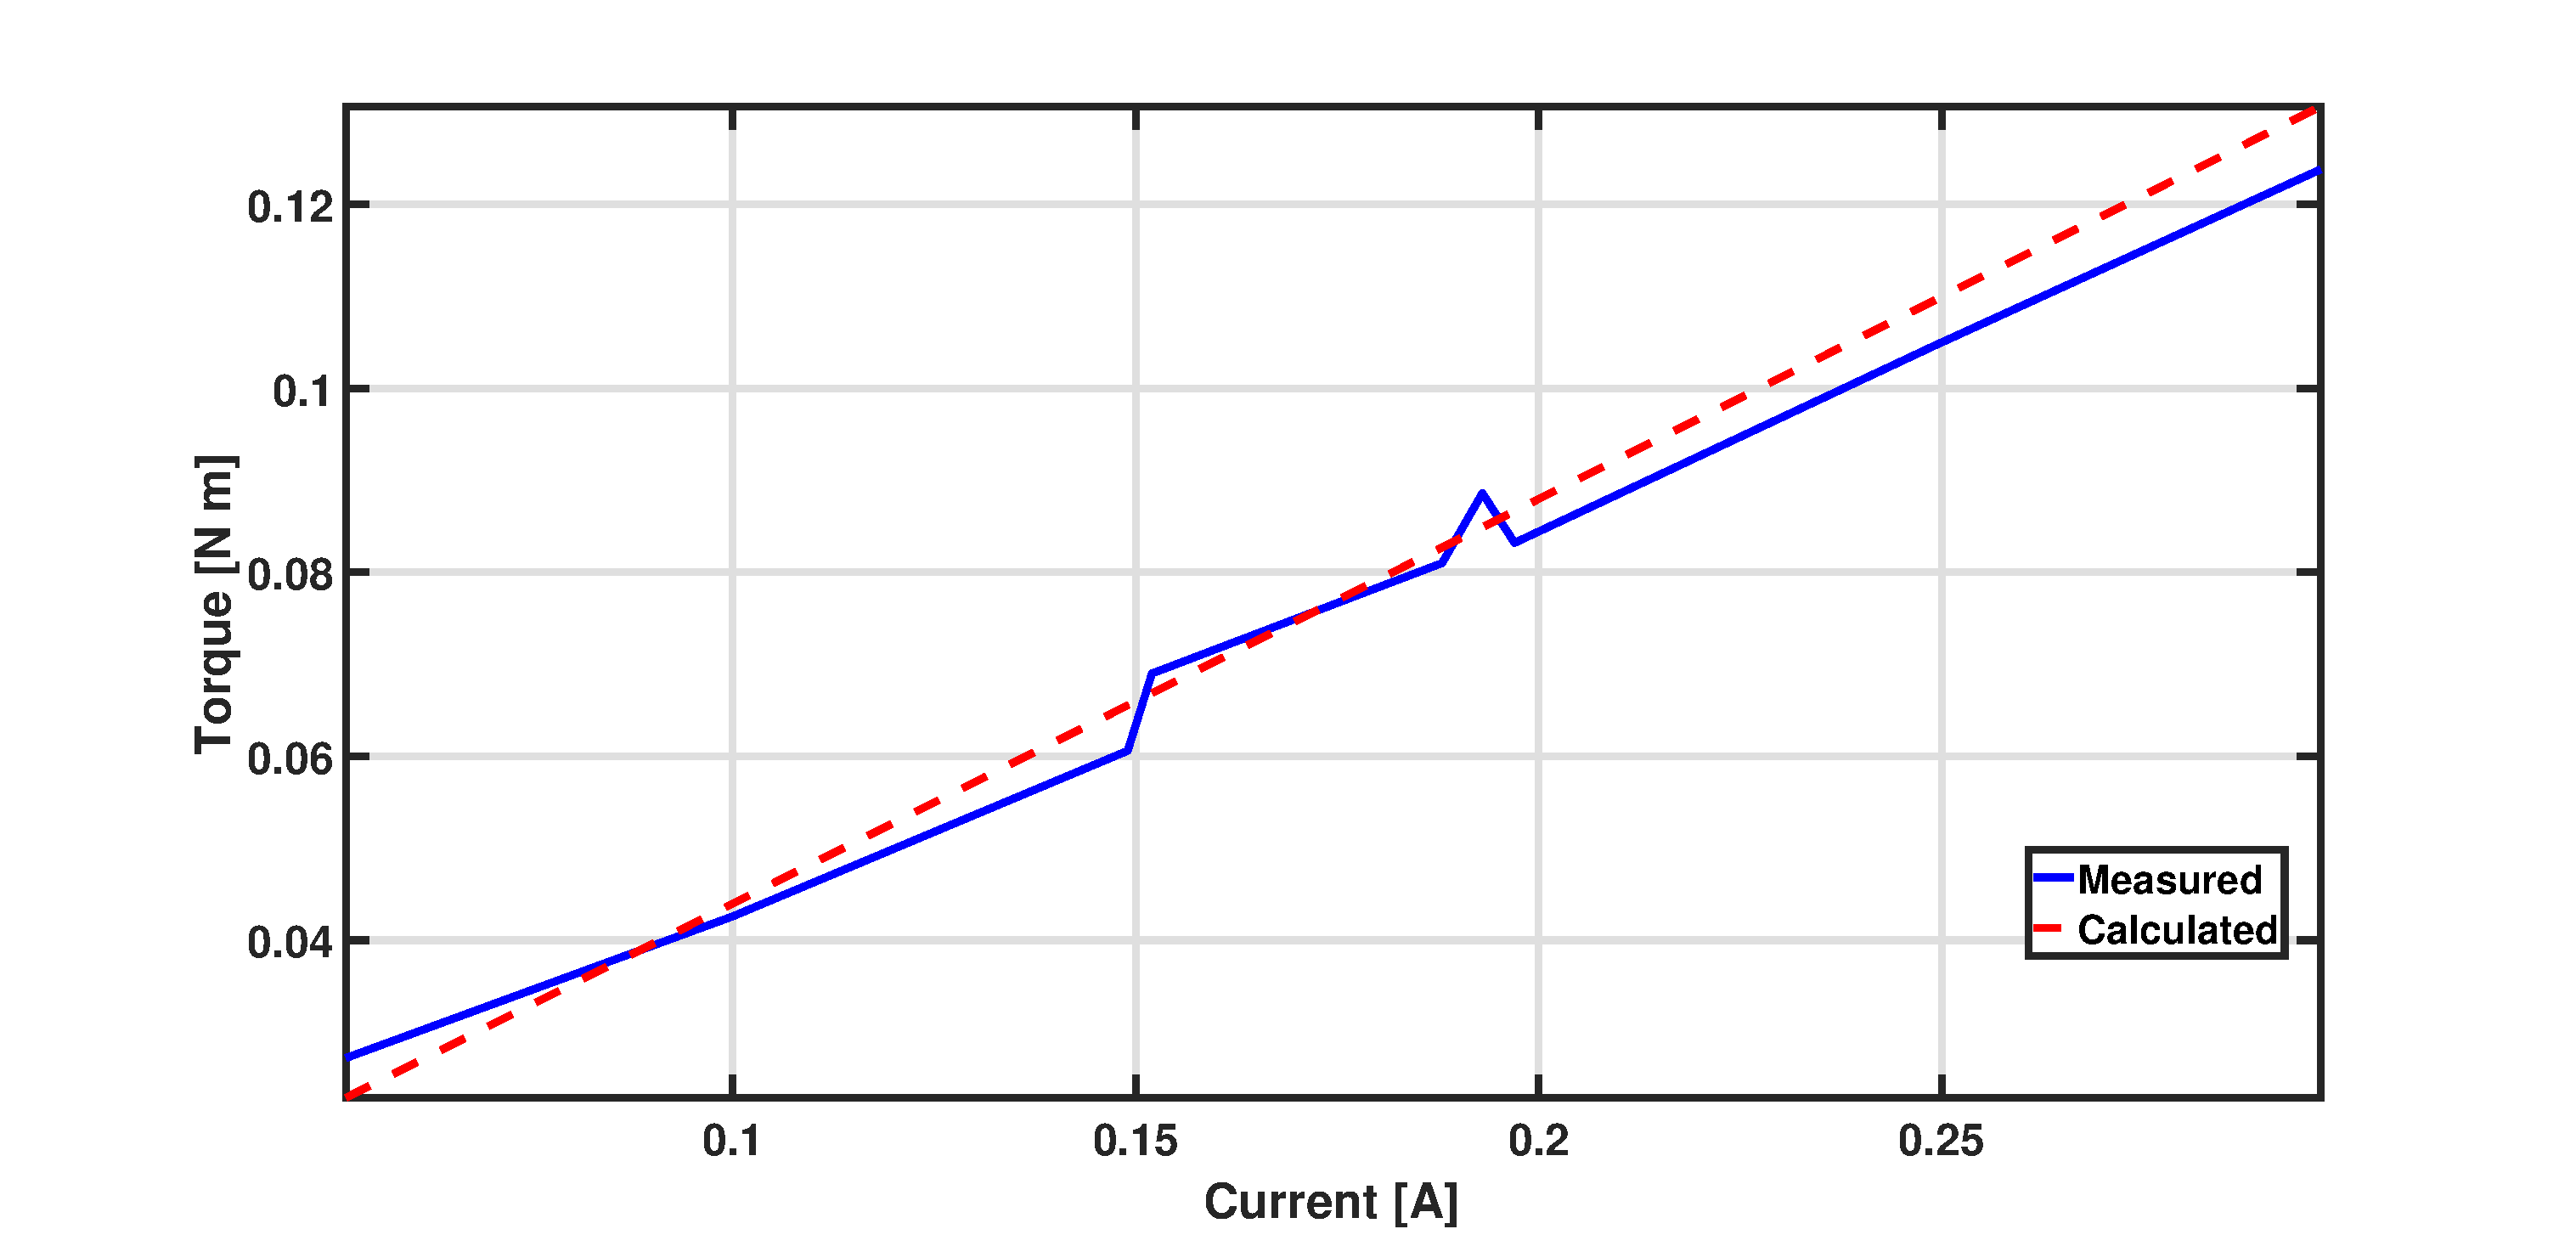
\includegraphics[width=\textwidth]{figures/test/MotorTorqueConstantMeasurement}
\caption{Graph of the torque $\tau_l(t)$ measured by the sensor, in respect to the motor current $i_a(t)$. The calculated torque is given by $\tau_m(t) = i_a(t) \cdot K_t$.}\label{fig:DCMotorKtMeasurement}
\end{figure}

It is seen that the current $i_a(t)$ and the torque $\tau_l(t)$ is approximately proportional as stated by \autoref{eq:AppendixDCMotorKtProportionality}. The average $K_t$ is calculated by \autoref{eq:AppendixDCMotorKtAverage}.
\begin{equation}
K_t\approx \frac{\sum\limits_{n=0}^{x-1} \frac{\tau_{l}[n]}{i_{a}[n]}}{x}=\SI{0.43}{\newton\metre\per\ampere}\label{eq:AppendixDCMotorKtAverage}
\end{equation}
\startexplain
\explain{$x$ is the number of measurements}{\noSIunit}
\explain{$n$ is the measurement number from 0 to $(x-1)$}{\noSIunit}
\stopexplain

Now that $K_t$ has been determined, the friction coefficient $B_m$ can be calculated.

\subsection*{Calculating $\boldsymbol{B_m}$}
When there is no load applied to the motors rotor shaft, and the system is in steady state, meaning $\frac{d \omega_{m}(t)}{d t} = 0$, \autoref{Appendix:BmCalculation1} can be derived.
\begin{equation}
0 = \tau_{m}(t) - B_m \cdot \omega_{m}(t)	\addunit{\newton\metre}\label{Appendix:BmCalculation1}
\end{equation}

From \autoref{eq:AppendixDCMotorKtProportionality} it is seen that $\tau_m(t) = i_a(t) \cdot K_t$, therefore \autoref{Appendix:BmCalculation2} can be written. 
\begin{subequations}
\begin{align}
B_m \cdot \omega_{m}(t)=i_a(t) \cdot K_t 	\addunit{\newton\metre\second\per\radian}\label{Appendix:BmCalculation2} \\
\implies B_m =\frac{i_a(t) \cdot K_t}{\omega_{m}(t)} \addunit{\newton\metre\second\per\radian} \label{Appendix:BmCalculation2.5}
\end{align}
\end{subequations} 

By using the results from \autoref{test:Ke}, the average $B_m$ can be calculated by \autoref{Appendix:BmCalculation3}.
\begin{equation}
B_m = \frac{\sum\limits_{n=0}^{x-1} \frac{i_{a}[n]\cdot K_t}{\omega_{m}[n]}}{x}=\SI{0.0009}{\newton\metre\second\per\radian}\label{Appendix:BmCalculation3}
\end{equation}

With the value of $B_m$, a resultant torque for a given angular frequency can be calculated. \autoref{fig:DCMotorBm} shows the torque given by the currents from \autoref{test:Ke} multiplied by $K_t$, compared to the torque calculated by $B_m$ and the angular velocity.
\begin{figure}[!h]
\centering
\includegraphics[width=\textwidth]{figures/test/MotorFrictionCoefficient}
\caption{Graph of the resultant torque from the friction in the motor in respect to the angular velocity of the motors rotor shaft. All measuremnets are done in steady state, meaning $\frac{d \omega_{m}(t)}{d t} = 0$.}\label{fig:DCMotorBm}
\end{figure}

From the graph is it seen that the measured values does not have the expected proportionality between the torque and the velocity. By inspection of the measured line, it is seen that it has a slight curvature and a constant element, meaning that it is nonlinear. It is however evaluated that approximating the friction as being linear is good enough for the project.

\newpage
\section*{Conclusion}
The result for the test and calculation for the DC motor torque constant $K_t$ is on average \SI{0.43}{\newton\metre\per\ampere} and the friction coefficient $B_m$ is on average \SI{0.0009}{\newton\metre\second\per\radian}.